\chapter{Protokoły}
	\section{IP}
%		\subsection{Opis}
			Protokół internetowy (ang. \textit{Internet Protocol}), jest protokołem działającym w trzeciej warstwie sieciowej modelu OSI - warstwie sieciowej.
			Odpowiedzialny jest za dostarczanie pakietów do hostów.
			Hosty używające protokołu IP są adresowane przy użyciu adresów IP.

			Aktualnie najpowszechniejszą wersją protokołu IP jest wersja IPv4, w której używany jest 32 bitowy adres.
			Drugą wersją, która zaczyna wypierać IPv4 jest wersja IPv6, w której adresy mają długość 128 bitów.

			Jeżeli wysyłane dane w pakiecie są większe niż MTU (\textit{MAximum Transfer Unit}), pakiet zostaje pofragmentowany, czyli podzielony na mniejsze porcje danych, tak aby ich rozmiar wraz z nagłówkiem były mniejsze niż najmniejsze MTU na trasie na której będzie przesyłany pakiet.
			W przypadku fragmentaryzacji pakietu, zostają ustawione odpowiednie flagi w pakiecie - szczegóły poniżej.
		\subsection{Nagłówek IP}
		%http://www.freesoft.org/CIE/Course/Section3/7.htm
			Każdy pakiet IP zostaje opakowany w ramkę IP.
			Schemat takiej ramki został pokazany na rys. \ref{fig:ramka_ip}.
			\begin{figure}[h]
				\centering
				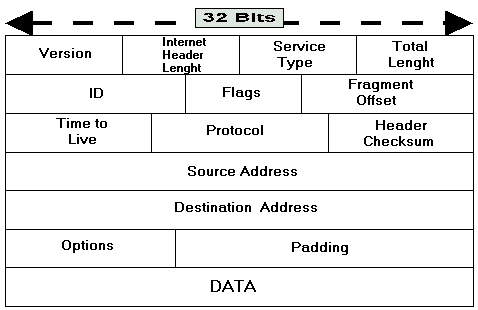
\includegraphics[width=400px]{ip.png}
				\caption{Ramka pakietu IP, źródło: \cite{headers}}
				%http://www.netguru.net/ntc/ntcgrap/Image53.gif
				\label{fig:ramka_ip}
			\end{figure}
			Znaczenie poszczenie poszczególnych pól jest następujące:
			\begin{description}
			\item[Version, 4bit]\hfill\\
				Determinuje która wersja protokołu IP będzie używana.
			\item[Internet Header Length, 4bit]\hfill\\
				Przechowuje informację o długości nagłówka IP.
				Wartość ta jest zawsze wielokrotnością 32 bitów.
				Aby nagłówek mógł być wielokrotnością 32 bitów, dodawana jest wartość pusta na końcu nagłówka, aby dopełnić jego długość do wielokrotności 32 bitów.
			\item[Service Type, 8bit]\hfill \\
				Przetrzymuje informacje o typie przesyłanych danych.
				Wartość ta była dawniej używana do profilowania ruchu (\textit{QoS}), jednak aktualnie jest ona najczęściej ignorowana przez routery.
			\item[Total Length, 16bit]\hfill \\
				Zawiera długość całego pakietu - nagłówka oraz danych.
			\item[ID, 16bit]\hfill \\
				Numer identyfikacyjny pakietu.
			\item[Flags, 3bit]\hfill\\
				Flagi pakietu.
				\begin{itemize}
					\item bit 0 - zarezerwowany
					\item bit 1 - DF - \textit{Don't fragment}, określa czy pakiet może być fragmentowany
					\item bit 2 - MF - \textit{More fragments}, określa czy będą następne fragmenty, czy ten jest ostatni
				\end{itemize}
			\item[Fragment Offset, 13bit]\hfill\\
				Określa w miejsce w datagramie w którym znajduje się dany fragment
			\item[Time to live, 8bit]\hfill\\
				Przechowuje wartość TTL, określającą długość życia pakietu.
				Wartość ta jest mierzona w ilości ruterów jakie może minąć pakiet, ponieważ na każdym ruterze wartość ta jest zmniejszana o 1.
				Jeżeli wartość spadnie do 0, router kasuje pakiet i odsyła do nadawcy informacje o przekroczeniu czasu życia pakietu.
			\item[Protocol, 8bit]\hfill\\
				Określa jaki protokół transportowy jest wykorzystywany przy połączeniu.
				Najpopularniejszymi protokołami są:
				\begin{itemize}
				%http://en.wikipedia.org/wiki/List_of_IP_protocol_numbers
					\item 0x04 - enkapsulacja IPv4
					\item 0x06 - TCP
					\item 0x01 - ICMP
					\item 0x11 - UDP
				\end{itemize}
			\item[Header Checksum, 16bit]\hfill \\
				Suma kontrolna nagłówka.
				Pozwala ona na kontrolowanie, czy nagłówek nie uległ zmianie przy przesyłaniu.
				Wartość ta jest sprawdzana i przeliczana na każdym routerze, ponieważ wartość TTL zostaje zmniejszana.
			\item[Source adres, 32bit]\hfill \\
				Zawiera adres źródłowy pakietu.
			\item[Destination address, 32bit]\hfill \\
				Zawiera adres docelowy pakietu.
			\item[Options]\hfill \\
				Zestaw różnych opcji pakietów IP.
				Ich opis jest poza zakresem tej pracy.
			\item[Padding]\hfill \\
				Dopełnienie nagłówka do pełnej wielokrotności 32 bitów.
				Wynika to z faktu, że wartość Internet Header Length zawiera długość nagłówkach w 32 bitowych słowach.
				Aby wartość ta miała prawo bytu, nagłówek musi być długości wielokrotności słowa.
			\end{description}	
	\section{TCP}
%		\subsection{Opis}
			TCP (ang. \textit{Transmission Control Protocol}) jest połączeniowym protokołem transportowym.
			Odpowiada on za nawiązywanie połączenia oraz jego kontrolowanie.

			Protokół TCP często jest protokołem transportowym dla IP.
			Razem tworzą najpowszechniejszą parę TCP/IP.
			Protokół IP używany jest jedynie do określania nadawcy pakietu, natomiast określanie usług docelowych leży po stronie TCP.\\

			Dodatkowo, protokół TCP oddziela różne równoległe strumienie danych pomiędzy dwa hostami.
			Wprowadza on, obok adresów IP źródłowych i docelowych z protokołu IP, porty - źródłowy i docelowy.
			Używając kwartetu parametrów, TCP jest wstanie jednoznacznie sprecyzować, do którego połączenia należy pakiet.\\
			Połączenie zwykle nawiązywane jest z losowego portu źródłowego (zwykle numer portu źródłowego jest większy niż 1024) na znany port docelowy.
			Numery portów poniżej 1024 są zarezerwowane dla tzw. \textit{Well known ports} czyli usług o zwyczajowo przypisanych stałych portach.
			Najważniejszymi dobrze znanymi portami są:
			\begin{itemize}
				\item 80 - WWW
				\item 110 - POP3
				\item 25 - SMTP
				\item 22 - SSH
				\item 21 - FTP
				\item 20 - FTP-DATA
				\item 23 - TELNET
			\end{itemize}
		\subsection{Nagłówek TCP}
			Każdy pakiet TCP zostaje opakowany w ramkę TCP.
			Schemat takiej ramki został pokazany na rys. \ref{fig:ramka_tcp}.
			\begin{figure}[h]
				\centering
				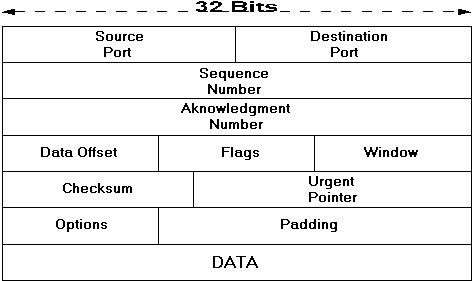
\includegraphics[width=400px]{tcp.png}
				\caption{Ramka pakietu TCP, źródło: \cite{headers}}
				%http://www.netguru.net/ntc/ntcgrap/Image54.gif
				\label{fig:ramka_tcp}
			\end{figure}
			Znaczenie poszczenie poszczególnych pól jest następujące:
			\begin{description}
			\item[Source Port, 16bit]\hfill \\
				Numer portu źródłowego.
			\item[Destination Port, 16bit]\hfill \\
				Numer portu docelowego.
			\item[Sequence Number, 32bit]\hfill \\
				Numer sekwencyjny pakietu.
			\item[Acknowledgment Number, 32bit]\hfill \\
				Numer sekwencyjny odpowiedzi.	
			\item[Data Offset, 4bit]\hfill \\
				Odległość od początku pakietu w którym zaczynają się dane.
				Wartość wyrażona w 32 bitowych słowach.
			\item[Flags, 9bit]\hfill \\
				Zawiera flagi cechujące dany pakiet TCP.
				Najważniejsze używane flagi to:
				\begin{itemize}
					\item SYN - oznacza pakiety przeprowadzające synchronizację numerów sekwencyjnych
					\item ACK - oznacza pakiety potwierdzające otrzymanie pakietów
					\item FIN - oznacza pakiet żądanie zakończenia połączenia
					\item RST - oznacza natychmiastowe resetowanie połączenia.
				\end{itemize}
			\item[Window, 16bit]\hfill \\
				Rozmiar okna. Mechanizm okna pozwala na kontrolowanie przepływu danych oraz przyśpieszenie wysyłania danych.
			\item[Checksum, 16bit]\hfill \\
				Suma kontrolna nagłówka. Pozwala sprawdzić czy nagłówek nie uległ modyfikacji podczas przesyłania.
%			\item[Urgent Pointer, 16bit]\hfill\\
%				\textcolor{red}{\Large{Nie rozumiem idei tego pola. Byłbym wdzięczny za pomoc}}
			\item[Options]\hfill\\
				Inne dodatkowe parametry cechujące pakiet
			\item[Padding]\hfill\\
				Dopełnienie nagłówka zerami do rozmiaru będącego wielokrotnością słowa.
			\end{description}
		\subsection{Nawiązywanie połączenia}
			Aby nawiązać połączenie przy użyciu protokołu TCP, należy przeprowadzić procedurę połączeniową, zwaną \textit{3 way handshake}, ponieważ, aby nawiązać połączenie, potrzeba wymienić trzy pakiety.\\
			Początkowo, host inicjujący połączenie, wysyła pakiet z ustawioną flagą SYN, oraz specjalnie wygenerowaną losową wartością pola SEQ. Host odbierający pakiet SYN, odpowiada pakietem z ustawionymi flagami SYN oraz ACK, oraz specjalnie wygenerowaną wartością losową SEQ, natomiast wartość pola ACK zawiera wartość SEQ z pakietu SYN powiększoną o 1.
			W odpowiedzi host inicjujący połączenie wysyła pakiet z flagą ACK oraz wartościami SEQ równej pierwszej wartości SEQ powiększonej o jeden, oraz ACK zawierająca wartość SEQ z pakietu SYN+ACK powiększoną o 1.\\
			Po wymienieniu tych trzech pakietów, połączenie zostaje nawiązane.
			Powyższy schemat wymiany został przedstawiony na rys. \ref{fig:tcp_syn}.
			\begin{figure}[h]
				\centering
					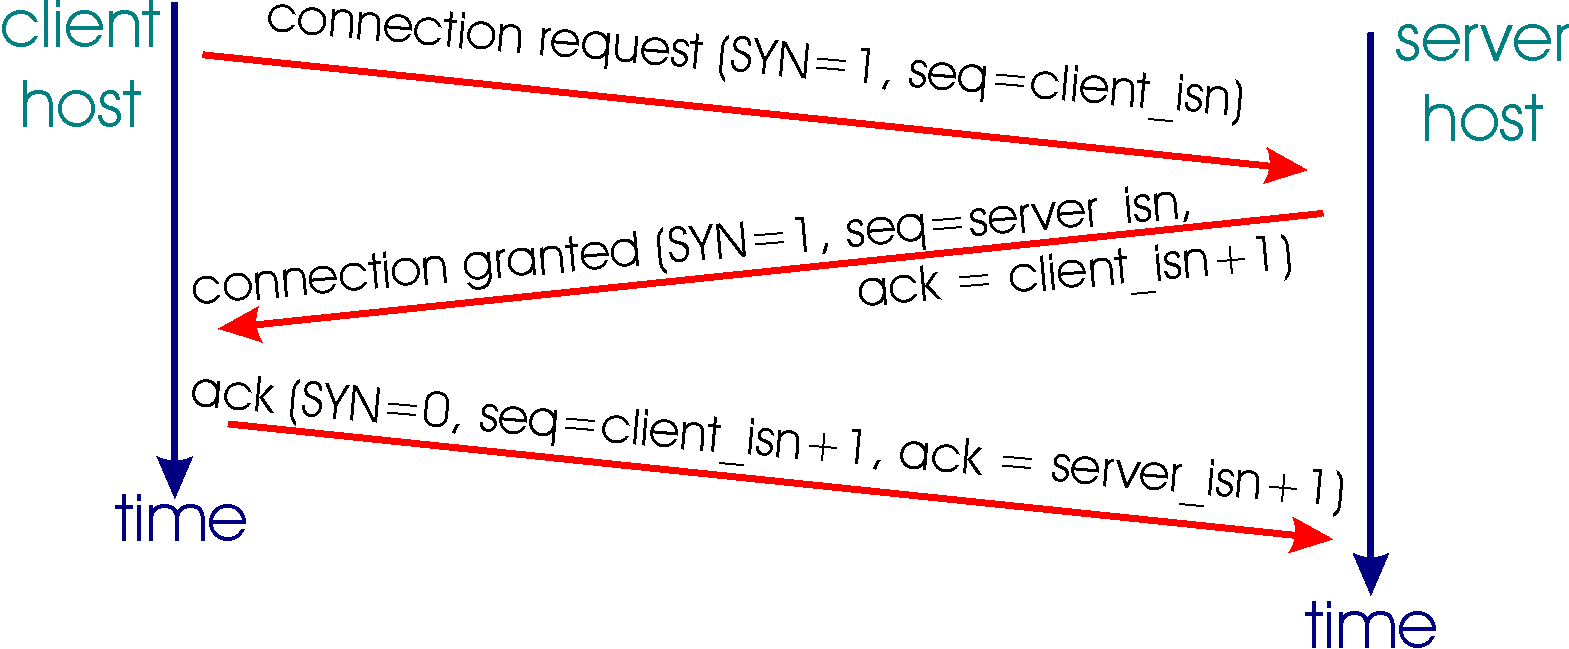
\includegraphics[width=400px]{tcp_3way.png}
					\caption{Nawiązywanie połączenia TCP, źródło: \cite{3way}}
					%http://www.bilgiagi.web.tr/wp-content/uploads/2011/03/tcp_3way.gif
					\label{fig:tcp_syn}
			\end{figure}
		\subsection{Kontrola transmisji}
			Protokół TCP kontroluje ciągłość transmisji poprzez numery sekwencyjne.
			Po nawiązaniu połączenia, każda ze stron połączenia ustaliła swoje numery sekwencyjne którymi będzie się posługiwać.
			
			Wysyłając pakiet o numerze sekwencyjnym 10, host odbierający wysyła pakiet ACK, z ustawionym numerem ACK równym numerowi sekwencyjnemu pakietu opowiadającemu temu potwierdzeniu.
			Host wysyłający, po otrzymaniu odpowiedzi ACK z numerem sekwencyjnym pakietu który wysłał, uznaje ten pakiet za dostarczony.\\
			W przypadku nie otrzymania odpowiedzi pewnym okresie czasu, uznaje się, że pakiet nie dotarł do adresata i następuje jego ponowne wysłanie.

			Przy wysyłaniu kolejnych pakietów, numery sekwencyjne zwiększane są o długość poprzedniego pakietu.
			Dla przykładu:\\
			Wysyłając pakiet o numerze sekwencyjnym 1000, oraz długości 100, otrzymamy odpowiedź z numerem ack równym 1000.
			Natomiast następny wysyłany pakiet będzie miał numer sekwencyjny 1100.
		\subsection{Mechanizm okna}
			Mechanizm przesuwnego okna pozwala na dopasowanie optymalnej prędkości przesyłu danych, przy zachowaniu ciągłości transmisji.

			Gdyby host wysyłający, po wysłaniu pakietu oczekiwał na potwierdzenie jego odebrania przez host docelowy, a następnie wysyłał kolejną porcję danych, otrzymalibyśmy w pełni stabilne połączenie, jednak odstępy pomiędzy wysyłaniem kolejnych pakietów były znaczne, ponieważ równe by były czasowi dotarcia pakietu do hosta docelowego oraz czasowi powrotu potwierdzenia.

			Aby tego uniknąć, host wysyłający mógłby wysyłać pakiety w serii, bez oczekiwania na potwierdzenia.
			Jednak, jeżeli host odbierający charakteryzuje się mniejszą mocą obliczeniową niż host wysyłający, nie będzie w stanie obsłużyć wszystkich dochodzących pakietów.
			Spowoduje to utratę tych pakietów i potrzeba ich retransmisji.
			Prowadzić to będzie do wielokrotnego wysyłania tych samych danych, co z efekcie spowoduje spadek prędkości połączenia.
		
			Używając mechanizmu okna, host wysyła pakiety w serii, tylko w rozmiarze nieprzekraczającym rozmiaru okna.
			Następnie zaprzestaje wysyłania pakietów, do chwili otrzymania potwierdzenia otrzymania pierwszego pakietu.
			Wtedy następuje przesunięcie okna o jedną pozycję i wysłanie kolejnego pakietu.\\
			Host docelowy odpowiada na odbierane pakiety, pakietami z wartościami ack równymi wartościom seq.
			W przypadku gdy host docelowy dostaje pakiet, którego parametr seq, jest większy niż wartość seq poprzedniego pakietu zsumowana z długością ostatniego pakietu, uznaje się, że w transmisji został zgubiony pakiet.
			Wtedy, host docelowy odpowiada wartością ack ostatniego poprawnego pakietu.
			Jeżeli zgubionym pakietem jest pierwszy pakiet w oknie nadawcy, okno nie zostaje przesunięte.
			W przypadku gdy host docelowy dostaje pakiet, którego parametr seq, jest większy niż wartość seq poprzedniego pakietu zsumowana z długością ostatniego pakietu, uznaje się, że w transmisji został zgubiony pakiet.
			Wtedy, host docelowy odpowiada wartością ack ostatniego poprawnego pakietu.
			Jeżeli zgubionym pakietem jest pierwszy pakiet w oknie nadawcy, okno nie zostaje przesunięte.
			Do hosta docelowego dostarczane są kolejne wysłane pakiety, na które odpowiedzią są pakiety z ack ostatniego poprawnego pakietu.
			Gdy nastąpi retransmisja zgubionego pakietu i retransmitowany pakiet zostanie dostarczony do hosta docelowego, ten odpowiada pakietem o ack ostatniego pakietu w serii. Dla przykładu:\\
			wielkość okna: 800
			\begin{itemize}\addtolength{\itemsep}{-1em}
			\item Host A $\rightarrow$ Host B: seq 1000, len 100
			\item Host A $\rightarrow$ Host B: seq 1100, len 100 (zagubiony)
			\item Host A $\rightarrow$ Host B: seq 1200, len 200
			\item Host A $\rightarrow$ Host B: seq 1400, len 100
			\item Host A $\rightarrow$ Host B: seq 1500, len 200
			\item Host A $\rightarrow$ Host B: seq 1700, len 100
			\item Host A $\leftarrow$ Host B: ack 1000 (odpowiedź na seq 1000)
			\item Host A $\rightarrow$ Host B: seq 1800, len 100
			\item Host A $\leftarrow$ Host B: ack 1000 (odpowiedź na seq 1200)
			\item Host A $\rightarrow$ Host B: seq 1100, len 100 (retransmisja)
			\item Host A $\leftarrow$ Host B: ack 1000 (odpowiedź na seq 1400)
			\item Host A $\leftarrow$ Host B: ack 1500 (odpowiedź na seq 1500)
			\item Host A $\rightarrow$ Host B: seq 1900, len 200
			\item Host A $\rightarrow$ Host B: seq 2100, len 100
			\end{itemize}
			Rozmiar okna jest ustalany dynamicznie w zależności o parametrów sieci i aktualnego obciążenia.
			Algorytmy ustalania jego wielkości są poza zakresem tej pracy.
		\subsection{Kończenie połączenia}
			Aby zakończyć połączenie, host wysyła pakiet z ustawioną flagą FIN oraz numerem sekwencyjnym równym SEQ.
			Host docelowy odpowiada pakietem ACK z wartością ack równą SEQ+1 otrzymanego pakietu.
			Następnie również wysyła pakiet FIN do hosta kończącego połączenie.
			Host kończący odpowiada pakietem ACK w wartością ack równą SEQ+1 pakietu FIN.
			Po wysłaniu ACK, host kończący uznaje połączenie za zakończone, natomiast host docelowy uznaje połączenie za zakończone po otrzymaniu ACK.
		\subsection{Nieoczekiwane zachowania}
			Protokół TCP reaguje na nieoczekiwane zachowania wysyłaniem pakietu z ustawioną flagą RST.
			Takimi nieoczekiwanymi sytuacjami mogą być:
			\begin{itemize}
			\item Wysłanie pakietu SYN na port na którym nie słucha żadna usługa.\\
				Jeżeli TCP otrzymuje pakiet SYN na porcie na którym nie słucha żadna usługa, uznaje, że taki pakiet nie jest oczekiwanym pakietem i odpowiada hostowi wysyłającemu pakietem z ustawionymi flagami RST i ACK.
				Jest to informacja że na tym porcie nie są oczekiwane połączenia.
			\item Wysłanie pakietu ACK.\\
				Jeżeli host otrzymuje nieoczekiwany pakiet ACK, wygenerowana zostaje informacja do hosta nadającego o zaprzestanie transmisji.
				Informacja taka jest przekazywana poprzez pakiet z ustawioną flagą RST.
			\end{itemize}

